\documentclass{article}
\usepackage[utf8]{inputenc}
\usepackage{graphicx}
\usepackage{color}

\title{Gray Laser Manual}
\author{Conrad Kuz}
\date{March 2022}

\begin{document}

\maketitle

\section{Introduction}
Basic guide for operating the GRAY laser.

\section{Regular Use Steps}
\begin{enumerate}
    \item Turn on water chiller
    \item Check vacuum pressure (Should be e-4)
    \item Turn oscillator to 3.5watts
    \item Modelock oscillator
    \item Turn switch and key on pump
    \item Activate timing computer
    \item Run pump on external
    \item Turn pockel cell on to 7kV
    \item Check that all beam lines are unblocked
    \item Check the output of the regen with a photodiode (DET210 Conrad thinks). You want the prepulse contrast to be 1:100 or better. If not, adjust the tip-tilt of the Pockel's cell and rotate the half waveplate slightly.
\end{enumerate}

\section{Regen alignment}
\begin{enumerate}
    \item Align pump to center of crystal. Run at low power and use lens tissue to see crystal.
          \begin{figure}[!ht]
              \centering
              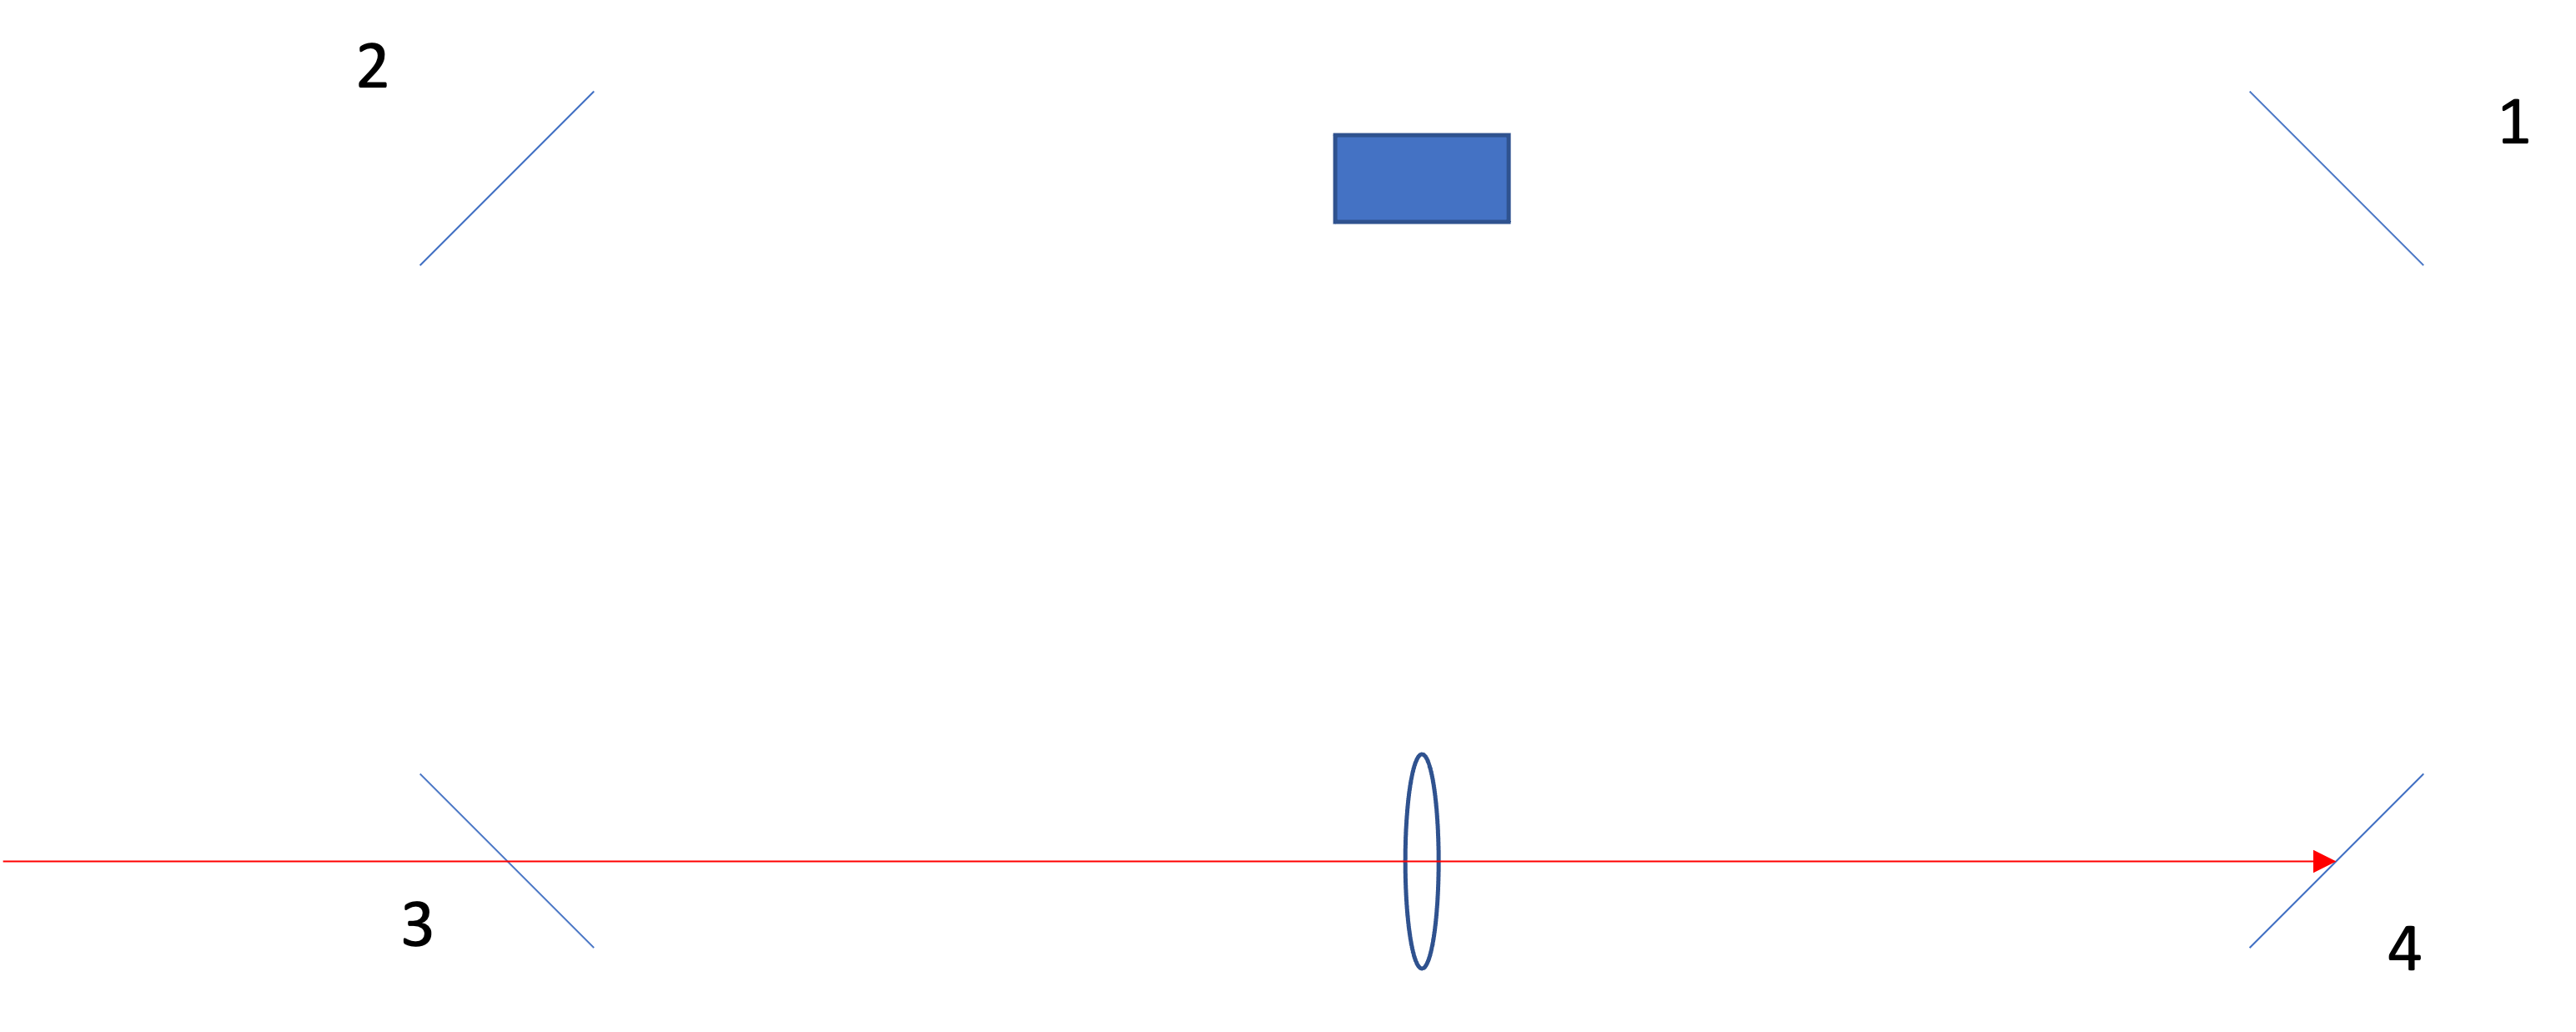
\includegraphics[width=1.0\textwidth]{Regen Alignment/HeNe Alignment}
              \caption{Setup for basic HeNe Alignment}
              \label{fig:HeNe_alignment}
          \end{figure}
    \item Send HeNe perpendicularly through lens and back mirrors.
    \item \label{itm:tweakCrystal} Tweak mirror 1 and 4 to send hene through center of crystal back face and front face. Use lens tissue to see crystal shadow
    \item \label{itm:tweakOverlap} Check overlap using lens tissue of forward and backward propagation between mirror 2 and crystal. Tweak mirror 3 until they are on top of each other.
    \item check overlap of forward and backward propagation between mirror 2 and 3. Tweak mirror 2 to correct. Repeat previous step until perfect on both sides
    \item \label{itm:optimizeAmps} Run pump at 24amps, check for lasing with IR viewer. Slightly tweak one of the four cavity mirrors while decreasing pump power to achieve lowest power with visible lasing.
    \item Install polarizers. Align for perfect back reflection then rotate each stage antiparallel by ~72 (Optimal angle for these polarizers) degrees
    \item Install waveplate, set to zero rotation
    \item Cross check step \ref{itm:tweakCrystal} and \ref{itm:tweakOverlap}
    \item Repeat step \ref{itm:optimizeAmps}, additionally, tweak waveplate for best lasing.
          \begin{figure}[!ht]
              \centering
              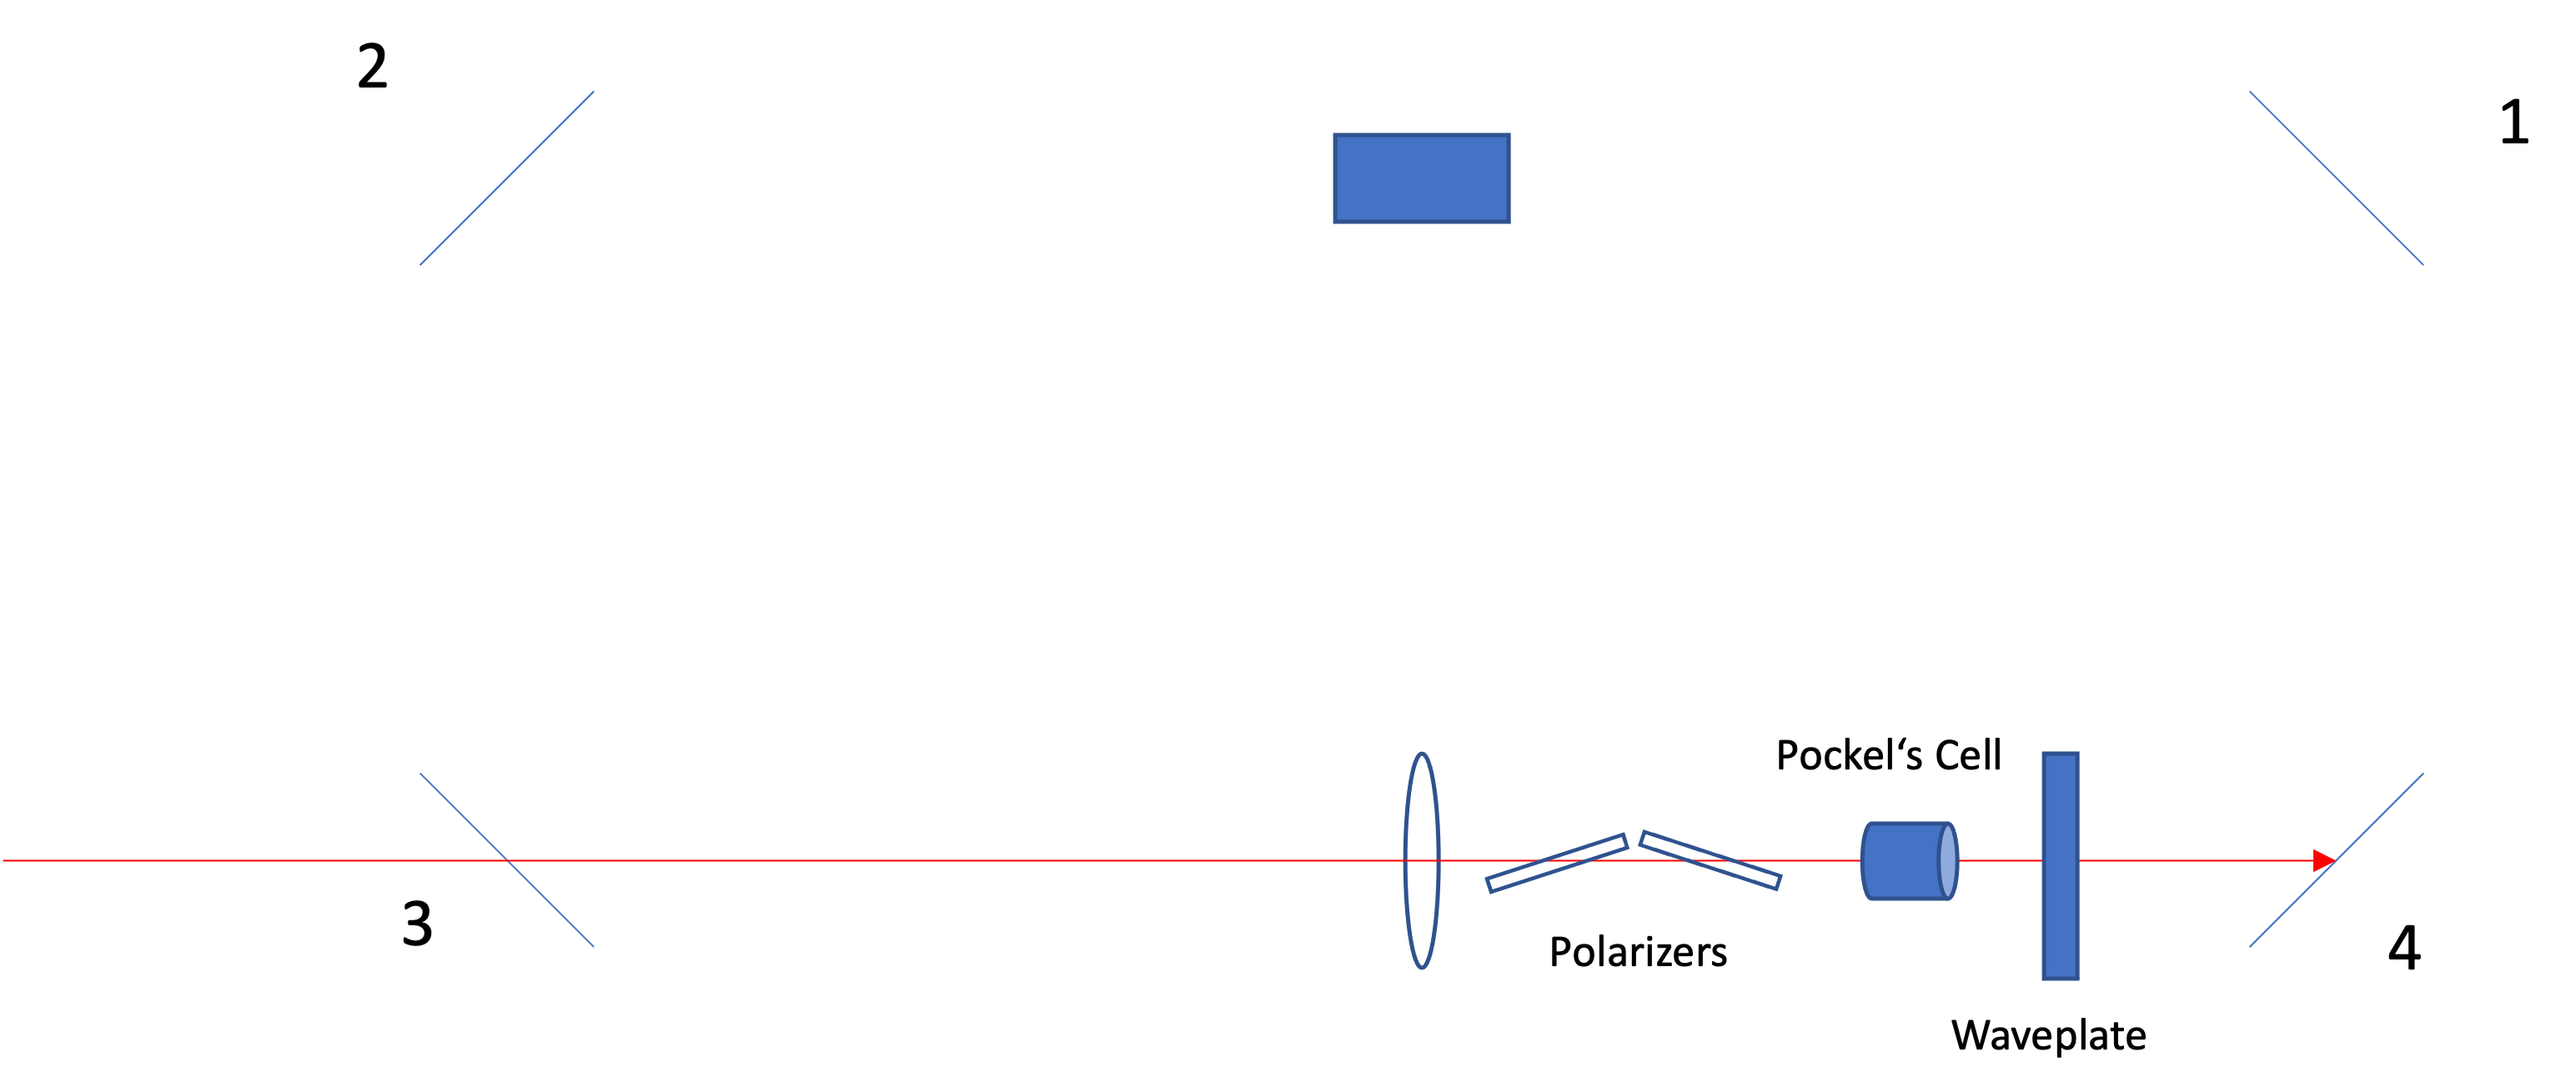
\includegraphics[width=1.0\textwidth]{Regen Alignment/PolarizerAlignment.png}
              \caption{Caption}
              \label{fig:polarizer_alignment}
          \end{figure}
    \item Install pockel's cell. Align beam through center then tweak alignment using dot and cross method - Maltese Cross.
    \item Repeat step \ref{itm:optimizeAmps}
    \item Place two irises in the lasing mode, one between mirror 2 and 3, and one between 1 and 4.
    \item Align the seed pulse to bounce off the polarizer closest to the lens so it follows the lasing mode. Use the two irises from the previous step.
    \item With waveplate at zero degree rotation, Pockel cell on maybe look at output on oscilliscope. Set pulse width to 0.6, delay around 3
    \item Tweak optics until good seeded gaussian with pulses touching zero volts.
    \item Set waveplate to 45 degrees past zero degree rotation mark
    \item set pockel pulse window to greater than 1.4 microsecond
    \item tweak wave plate
    \item tweak pockel delay until most power
    \item decrease pockel pulse window to dump on one pulse
    \item tweak optics to optimize power
\end{enumerate}
\section{Regen Timing}
Oscillator creates 76MHz pulse detected by a photodiode

\section{Compressor Alignment}
\begin{enumerate}
    \item Align regen output to compressor telescope.
    \item Install two tall irises and align the beam after the periscope to them.
    \item run d-scan and auto-correlation. adjust as necessary
\end{enumerate}

\section{Fixing Oscillator}
Over time, the oscillator cavity will tend to drift, such that CW power may drop from 400mW to something like 300mW or worse.
In that case, the cavity mirrors {\color{red} add annotated picture} need to be adjusted to maximize the CW power.
When the CW power falls, modelocking will either become impossible, or if modelocking is achieved, it will be unstable and randomly drop out.

\section{Troubleshooting dumb stuff}
\begin{itemize}
    \item When using oscilliscope, check BNC is connected.
    \item Make sure seed is unblocked
\end{itemize}




\end{document}
